    
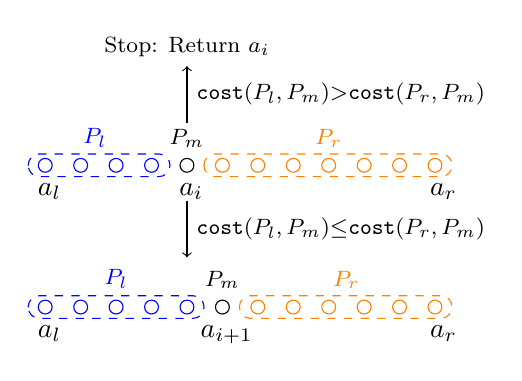
\begin{tikzpicture}[scale = 1.8]

%\draw[help lines, color=gray!30, dashed] (-1,-2) grid (4.9,1);
\node[circle,draw=blue, fill=white, inner sep=0pt,minimum size=5pt] (b) at (-1,0) {};
\node[circle,draw=blue, fill=white, inner sep=0pt,minimum size=5pt] (b) at (-0.25,0) {};
\node[circle,draw=blue, fill=white, inner sep=0pt,minimum size=5pt] (b) at (-0.5,0) {};
\node[circle,draw=blue, fill=white, inner sep=0pt,minimum size=5pt] (b) at (-0.75,0) {};
\node[circle,draw=black, fill=white, inner sep=0pt,minimum size=5pt] (b) at (0,0) {};
\node[circle,draw=orange, fill=white, inner sep=0pt,minimum size=5pt] (b) at (0.25,0) {};
\node[circle,draw=orange, fill=white, inner sep=0pt,minimum size=5pt] (b) at (0.5,0) {};
\node[circle,draw=orange, fill=white, inner sep=0pt,minimum size=5pt] (b) at (0.75,0) {};
\node[circle,draw=orange, fill=white, inner sep=0pt,minimum size=5pt] (b) at (1,0) {};
\node[circle,draw=orange, fill=white, inner sep=0pt,minimum size=5pt] (b) at (1.25,0) {};
\node[circle,draw=orange, fill=white, inner sep=0pt,minimum size=5pt] (b) at (1.5,0) {};
\node[circle,draw=orange, fill=white, inner sep=0pt,minimum size=5pt] (b) at (1.75,0) {};
\node[below]  at (-0.97,-0.06) {$a_l$};
\node[below]  at (1.81,-0.06) {$a_r$};
\node[below]  at (0.03,-0.06) {$a_i$};
\node[above, color=blue]  at (-0.65,0.06) {\footnotesize{{$P_l$}}};
\node[above, color=orange]  at (1,0.06) {\footnotesize{{$P_r$}}};
\node[above, color=black]  at (0,0.06) {\footnotesize{{$P_m$}}};
\draw[->] (0,0.3)--(0,0.7);
\node[right, color=black]  at (0,0.5) {\footnotesize{\texttt{cost}($P_l,P_m$)$>$\texttt{cost}($P_r,P_m$)}};
\node[above, color=black]  at (0,0.7) {\footnotesize{Stop: Return $a_i$}};
\draw [blue, dashed,rounded corners] (-1.12,-0.08) rectangle (-0.12,0.08);
\draw [orange, dashed,rounded corners] (0.12,-0.08) rectangle (1.87,0.08);
\draw[->] (0,-0.25)--(0,-0.65);
\node[right, color=black]  at (0,-0.45) {\footnotesize{\texttt{cost}($P_l,P_m$)$\leq$\texttt{cost}($P_r,P_m$)}};
\node[circle,draw=blue, fill=white, inner sep=0pt,minimum size=5pt] (b) at (-1,-1) {};
\node[circle,draw=blue, fill=white, inner sep=0pt,minimum size=5pt] (b) at (-0.25,-1) {};
\node[circle,draw=blue, fill=white, inner sep=0pt,minimum size=5pt] (b) at (-0.5,-1) {};
\node[circle,draw=blue, fill=white, inner sep=0pt,minimum size=5pt] (b) at (-0.75,-1) {};
\node[circle,draw=blue, fill=white, inner sep=0pt,minimum size=5pt] (b) at (0,-1) {};
\node[circle,draw=black, fill=white, inner sep=0pt,minimum size=5pt] (b) at (0.25,-1) {};
\node[circle,draw=orange, fill=white, inner sep=0pt,minimum size=5pt] (b) at (0.5,-1) {};
\node[circle,draw=orange, fill=white, inner sep=0pt,minimum size=5pt] (b) at (0.75,-1) {};
\node[circle,draw=orange, fill=white, inner sep=0pt,minimum size=5pt] (b) at (1,-1) {};
\node[circle,draw=orange, fill=white, inner sep=0pt,minimum size=5pt] (b) at (1.25,-1) {};
\node[circle,draw=orange, fill=white, inner sep=0pt,minimum size=5pt] (b) at (1.5,-1) {};
\node[circle,draw=orange, fill=white, inner sep=0pt,minimum size=5pt] (b) at (1.75,-1) {};
\node[below]  at (-0.97,-1.06) {$a_l$};
\node[below]  at (1.81,-1.06) {$a_r$};
\node[below]  at (0.28,-1.06) {$a_{i+1}$};
\node[above, color=blue]  at (-0.50,-0.94) {\footnotesize{{$P_l$}}};
\node[above, color=orange]  at (1.125,-0.94) {\footnotesize{{$P_r$}}};
\node[above, color=black]  at (0.25,-0.94) {\footnotesize{{$P_m$}}};
\draw [blue, dashed,rounded corners] (-1.12,-1.08) rectangle (0.12,-0.92);
\draw [orange, dashed,rounded corners] (0.37,-1.08) rectangle (1.87,-0.92);
\end{tikzpicture}